\documentclass[a4paper,12pt]{report}
\usepackage[margin=1in]{geometry} % 1-inch margins
\usepackage{tikz} % For the border
\usetikzlibrary{calc} % For coordinate calculations
\usepackage{graphicx} % For including the logo
\usepackage{lmodern} % Font package
\usepackage{titlesec} % Section formatting
\usepackage{fancyhdr} % Footer customization
\usepackage{amsmath}
\usepackage{listings}
\usepackage{caption}
\usepackage{subcaption}
\usepackage{geometry}
\usepackage{array}
\usepackage{booktabs}
\usepackage{makecell}
\usepackage{float}
\usepackage{tocloft}
\usepackage[colorlinks=true, linkcolor=black, citecolor=black, urlcolor=black]{hyperref}
\usepackage{lipsum}
\usepackage{adjustbox} % trong phần preamble
\usepackage{multicol}
\usepackage{indentfirst}
\usepackage{setspace}
\usepackage{textcomp} % để dùng ký hiệu độ





\pagestyle{fancy}
\lhead{Flight Delay Prediction}
\definecolor{codegreen}{rgb}{0,0.6,0}
\definecolor{codegray}{rgb}{0.5,0.5,0.5}
\definecolor{codepurple}{rgb}{0.58,0,0.82}
\definecolor{backcolour}{rgb}{0.95,0.95,0.92}
\setlength{\parskip}{0.2cm}  % khoảng cách giữa các đoạn là 0.2em

\lstdefinestyle{mystyle}{
    backgroundcolor=\color{backcolour},   
    commentstyle=\color{codegreen},
    keywordstyle=\color{magenta},
    numberstyle=\tiny\color{codegray},
    stringstyle=\color{codepurple},
    basicstyle=\ttfamily\footnotesize,
    breakatwhitespace=false,         
    breaklines=true,                 
    captionpos=b,                    
    keepspaces=true,                 
    numbers=left,                    
    numbersep=5pt,  
    showlines=false,
    showspaces=false,                
    showstringspaces=false,
    showtabs=false,                  
    tabsize=2
}


\lstset{ % Tùy chỉnh các thuộc tính
    basicstyle=\ttfamily\small, % Kiểu chữ máy tính nhỏ
    backgroundcolor=\color{lightgray}, % Màu nền nhẹ cho code
    keywordstyle=\color{blue}\bfseries, % Màu xanh dương cho từ khóa, in đậm
    commentstyle=\color{green}, % Màu xanh lá cho comment
    stringstyle=\color{purple}, % Màu tím cho chuỗi
    numberstyle=\tiny\color{gray}, % Màu xám cho số dòng
    numbers=left, % Hiển thị số dòng bên trái
    stepnumber=1, % Đánh số mỗi dòng
    numbersep=5pt, % Khoảng cách giữa số dòng và mã
    showstringspaces=false, % Không hiển thị dấu cách trong chuỗi
    breaklines=true, % Ngắt dòng tự động
    captionpos=b, % Đặt caption ở dưới code
    frame=single, % Đặt khung xung quanh code
}



\begin{document}
\thispagestyle{empty}  % Xóa số trang của trang đầu tiên

% --- First Page Border ---
\begin{tikzpicture}[remember picture, overlay]
    \draw[line width=2pt]
        ($(current page.south west) + (0.5in, 0.5in)$) 
        rectangle 
        ($(current page.north east) - (0.5in, 0.5in)$);
\end{tikzpicture}

% --- University Name ---
\begin{center}
    
    {\Large \textbf{University of Science and Technology of Hanoi}}\\[0.75cm]
    
    % --- University Logo ---
    
\begin{center}
  \makebox[\textwidth][c]{%
    \hspace*{1.2cm} % dịch logo sang trái 1cm, bạn thử chỉnh -0.8cm hoặc -1.2cm nếu cần
    
\includegraphics[width=0.7\textwidth]{Img/usth.png}%
  }
\end{center}

    
    \vspace{1cm}
    {\LARGE \textbf{Fundamentals of Data Science}}\\[0.75cm]

    % --- Assignment Title ---
    \vspace{0.5cm} % khoảng cách trước Labwork I
    {\huge
    \begin{spacing}{1.2} % tăng khoảng cách giữa các dòng lên 1.2 lần
    \textbf{A Data-Driven Approach to Predicting Flight Delays}
    
\end{spacing}
}
    \vspace{1.5cm} % khoảng cách sau Labwork I
\end{center}

% --- Student Information ---
\vspace{0.5cm}
\noindent
\begin{center}

    \begin{tabular}{l c r}
    
        \textbf{\large Group Members:}
        \vspace{0.5cm}
        \\
        \textbf{Nguyen Tuan Thanh} & 22BA13289 & thanhnt.22ba13289@usth.edu.vn
        \vspace{0.1cm}\\
        \textbf{Nguyen Chi Quang} & 22BA13262 & quangnc.22ba13262@usth.edu.vn \\
    \end{tabular}
\end{center}

\vfill

% --- Footer ---
\begin{center}
    \textit{Hanoi, Oct 2025}
\end{center}
\newpage
\pagenumbering{arabic} 
\setcounter{page}{2}  

% Đặt lại số trang về 1 cho mục lục và các phần sau

\tableofcontents  % Tạo mục lục tự động
\newpage
\listoffigures        % Mục lục các hình (Figures)
\listoftables         % (Nếu có bảng, thêm mục lục bảng)

\newpage

% ---------------- DÀN Ý ----------------
\chapter*{ACKNOWLEDGEMENTS}
We would like to express our sincere gratitude to our supervisor, Nguyen Duc Dung, for their valuable guidance, feedback, and continuous encouragement throughout the development of this project. Their insights greatly helped us refine our approach and achieve meaningful results.

We also appreciate the support from our peers and colleagues who provided constructive discussions and suggestions during the research process. Their perspectives enriched our understanding of the subject matter.
\addcontentsline{toc}{chapter}{ACKNOWLEDGEMENTS}

\chapter*{ABSTRACT}
Flight delays pose a significant operational and economic challenge for the aviation industry, affecting both airline efficiency and passenger experience. This project examines the factors influencing flight departure delays by integrating historical flight records with meteorological data for major airports in Washington State. A data engineering pipeline was developed to collect, clean, and merge data from the Bureau of Transportation Statistics (BTS) and the National Oceanic and Atmospheric Administration (NOAA). After comprehensive preprocessing and feature engineering, several machine learning models were employed to analyze delay patterns and identify key predictors. Statistical analysis and visualization techniques were applied to explore relationships between time, weather, and route characteristics under different delay scenarios. The findings provide insights into the underlying dynamics of flight delays and demonstrate how data-driven approaches can enhance predictive capability and operational decision-making in the aviation sector.
\vspace{0.5cm}

\noindent\textbf{Keywords:} \textit{Flight Delay Prediction, Data Engineering, Machine Learning, Weather Integration, Statistical Analysis, Feature Engineering, Aviation Analytics.}
\addcontentsline{toc}{chapter}{ABSTRACT}

\chapter{Introduction}
\section{Background}
Flight delays remain a major challenge in the aviation industry, affecting operational efficiency and passenger satisfaction. With increasing air traffic and weather variability, understanding and predicting delays has become essential for airlines and authorities. The integration of data science enables a deeper analysis of historical patterns and factors influencing flight punctuality.

\section{Problem Statement}
Flight operations are influenced by multiple interacting factors such as weather, route, schedule, and carrier performance. These factors do not act independently but combine in complex and nonlinear ways, making delay prediction a challenging task.

Traditional methods — such as basic statistical analysis or simple linear regression — mainly capture one-to-one, linear relationships between variables. However, they fail to represent nonlinear interactions among multiple operational and environmental features, limiting their ability to model real-world flight behaviors.

Therefore, this study aims to identify the key determinants of departure delays and to develop data-driven models capable of capturing these complex dependencies.

\section{Analytical Approach}
The project integrates flight and weather datasets from the Bureau of Transportation Statistics (BTS) and NOAA. After cleaning and merging, a machine-learning pipeline was applied to model departure delays. Techniques such as correlation analysis, feature engineering, and classification algorithms were used to uncover delay patterns.

\section{Goals and Implications}
The goal of this study is to build a data-driven analytical framework capable of predicting flight departure delays and identifying their main causes. By integrating flight and weather data into a unified dataset, the project applies machine-learning models to uncover delay patterns and key influencing factors. 

The outcomes of this analysis can support airlines and regulators in improving scheduling, resource allocation, and passenger communication. Through data-driven insights, this approach enhances the reliability and efficiency of air transport operations.


\chapter{Data Collection and Preparation}
\section{Introduction}
This project uses two complementary datasets: flight operation records and hourly weather observations. Combining operational and environmental data provides a more realistic view of factors influencing flight delays. Each dataset was individually cleaned and then merged into a unified analytical dataset for subsequent analysis and modeling.
\subsection{Flight Dataset}
The flight dataset used in this project is the \textbf{Airline On-Time Performance Data}, obtained from the \textbf{U.S. Bureau of Transportation Statistics}, which provides detailed records of domestic flight operations across the United States. This dataset serves as the primary source for analyzing operational factors contributing to departure delays.

For this study, only flights departing from Washington State during the second quarter (Q2) were used.
The dataset consists of 65,374 entries and 17 features, and is provided in CSV format.

The data types and detailed discussion of each feature in the dataset are provided below:


\begin{table}[H]
\centering
\begin{adjustbox}{width=\textwidth}
\begin{tabular}{|c|c|c|l|}
\hline
\textbf{Features} & \textbf{Type} & \textbf{Data Type} & \textbf{Explanation}\\
\hline
MONTH & Temporal & Integer & Month of the flight date. \\ 
\hline
DAY\_OF\_MONTH & Temporal & Integer & Day of the month. \\ 
\hline
DAY\_OF\_WEEK & Temporal & Integer & Day of the week. \\ 
\hline
OP\_UNIQUE\_CARRIER & Categorical & String & Unique carrier code identifying the airline. \\ 
\hline
ORIGIN & Categorical & String & Code of the departure (origin) airport. \\ 
\hline
ORIGIN\_STATE\_ABR & Categorical & String & Two-letter abbreviation of the origin state. \\ 
\hline
DEST & Categorical & String & Code of the arrival (destination) airport. \\ 
\hline
DEST\_STATE\_ABR & Categorical & String & Two-letter abbreviation of the destination state. \\ 
\hline
CRS\_DEP\_TIME & Temporal & Integer & Scheduled departure time (in HHMM format). \\ 
\hline
CRS\_ARR\_TIME & Temporal & Integer & Scheduled arrival time (in HHMM format). \\ 
\hline
CANCELLED & Quantitative (Binary) & Float & Indicates if the flight was cancelled (1 = Yes, 0 = No). \\ 
\hline
CRS\_ELAPSED\_TIME & Quantitative & Float & Scheduled flight time in minutes. \\ 
\hline
DISTANCE & Quantitative & Float & Distance between origin and destination airports (in miles). \\ 
\hline
DISTANCE\_GROUP & Categorical (Ordinal) & Integer & Group number representing distance range. \\ 
\hline
DEP\_DELAY & Quantitative & Float & Difference between actual and scheduled departure time. \\ 
\hline
DEP\_DEL15 & Quantitative (Binary) & Integer & 1 if departure delay > 15 minutes, otherwise 0. \\ 
\hline
DEP\_DELAY\_GROUP & Categorical (Ordinal) & Float & Grouping of departure delay intervals. \\ 
\hline
\end{tabular}
\end{adjustbox}
\caption{Features Explanation}
\end{table}
\subsection{Weather Dataset}
The weather dataset used in this project was obtained from the \textbf{National Oceanic and Atmospheric Administration (NOAA)}, which provides historical hourly weather observations recorded at airports across the United States. To ensure consistency with the flight dataset, only data from major airports in Washington State during the second quarter (Q2) were collected. The dataset contains over 50,000 hourly records with many key meteorological, stored in CSV format.

The data types and detailed discussion of each feature in the dataset are provided below:
\begin{table}[H]
\centering
\begin{adjustbox}{width=\textwidth}
\begin{tabular}{|c|c|c|l|}
\hline
STATION & Categorical & String & Identifier code where the weather data was recorded. \\ 
\hline
DATE & Temporal & Datetime & Timestamp representing the date and hour of the observation. \\ 
\hline
HourlyDewPointTemperature & Quantitative & Float & Dew point temperature (°F). \\ 
\hline
HourlyDryBulbTemperature & Quantitative & Float & Air temperature (°F). \\ 
\hline
HourlyRelativeHumidity & Quantitative & Float & Percentage of relative humidity in the air (\%). \\ 
\hline
HourlyVisibility & Quantitative & Float & Horizontal visibility distance (miles). \\ 
\hline
HourlyWindSpeed & Quantitative & Float & Average wind speed during the hour (miles per hour). \\ 
\hline
\end{tabular}
\end{adjustbox}
\caption{Features Explanation}
\end{table}

\section{Data Preparation and Cleaning}
\subsection*{Flight Data Cleaning and Preprocessing}

To ensure the data is suitable for analysis and modeling, several preprocessing steps were performed:

\begin{itemize}
    \item \textbf{Filtering by Origin State:}
    \begin{itemize}
        \item Kept only flights with \texttt{ORIGIN\_STATE\_ABR = 'WA'}, since the state has five main airports, which simplifies merging with weather data.
    \end{itemize}

    \item \textbf{Handling Missing and Duplicate Records:}
    \begin{itemize}
        \item Removed all rows with missing or zero values, except for time-related variables (\texttt{DEP\_DELAY}, \texttt{DEP\_DEL15}, \texttt{DEP\_DELAY\_GROUP}, \texttt{DEP\_DELAY\_NEW}).
        \item Identified and removed duplicate records.
    \end{itemize}

    \item \textbf{Removing Cancelled Flights:}
    \begin{itemize}
        \item Filtered out all cancelled flights (\texttt{CANCELLED = 1}) to focus on actual departure delays and removed \texttt{CANCELLED} column.
    \end{itemize}

    \item \textbf{Time Transformation:}
    \begin{itemize}
        \item Converted \texttt{CRS\_DEP\_TIME} and \texttt{CRS\_ARR\_TIME} from HHMM to decimal-hour format.
    \end{itemize}

    \item \textbf{General Summary:}
    \begin{itemize}
        \item After preprocessing, the dataset contains 17 features and 50,186 samples.
        \item The dataset is ready for merging and analysis.
    \end{itemize}
\end{itemize}

\subsection{Weather Data Cleaning and Preprocessing}
The weather dataset was cleaned and standardized to ensure accuracy and consistency before merging with the flight data.
\begin{itemize}
    \item \textbf{Handling Missing and Duplicate Records:}
    \begin{itemize}
        \item{Removed records containing NULL values.}
        \item{Duplicate records were identified and removed.}
    \end{itemize}
    \item \textbf{Extract new features:}
    \begin{itemize}
        \item{Converted the \texttt{DATE} column to datetime format.}
        \item {Extracted the day and month information into a new column date, formatted as “MM-DD” for easier temporal alignment.}
        \item {Extracted the hour component into a new column hour.}
    \end{itemize}
    \item \textbf{Map airport codes:}
    \begin{itemize}
        \item{The \texttt{STATION} codes were mapped from NOAA station IDs to corresponding airport IATA codes to ensure consistency with the flight dataset during merging.}
    \end{itemize}
    \item \textbf{General:}
    \begin{itemize}
        \item{After prepareing, dataset have 8 features and 10851 samples.}
        \item {Dataset is ready for merging and analysis.}
    \end{itemize}
\end{itemize}
\subsection{Merging Datasets}
After cleaning and preprocessing both datasets, they were merged to create a comprehensive dataset for analysis:
\begin{itemize}
    \item \textbf{Prepare Time Columns:}
    \begin{itemize}
        \item{Extracted the departure hour (\texttt{DEP\_HOUR}) from \texttt{CRS\_DEP\_TIME} by flooring the scheduled time to the nearest hour.}
        \item {Created a new column \texttt{FL\_DATE} by combining \texttt{MONTH} and \texttt{DAY\_OF\_MONTH}, with the year temporarily set to 2025.}
        \item {In the weather dataset, added the year “2025” to the date column (if missing) and converted it to datetime format.}
        \item {These transformations standardized date and time formats across both datasets, enabling accurate merging by hour and location.}
    \end{itemize}
    \item \textbf{Merge Flight \& Weather Data}
    \begin{itemize}
        \item{Merged flight and weather datasets using a left join on matching keys:
    \texttt{ORIGIN, FL\_DATE, DEP\_HOUR} $\rightarrow$ \texttt{STATION, date, hour}.}
        \item{Ensured each flight matched its corresponding hourly weather record.}
        \item {Removed intermediate columns that were no longer needed: ["\texttt{DEP\_HOUR}", "\texttt{FL\_DATE}", "\texttt{STATION}", "\texttt{date}", "\texttt{hour}"].}
    \end{itemize}
\end{itemize}

\begin{table}[H]
\centering
\begin{adjustbox}{width=\textwidth}
\begin{tabular}{|c|c|c|c|c|c|c|c|c|c|c|}
\hline
\textbf{MONTH} & \textbf{DAY\_OF\_MONTH} & \textbf{ORIGIN} & \textbf{HourlyVisibility} & \textbf{HourlyWindSpeed} & \textbf{...} & \textbf{DEST} & \textbf{DISTANCE} & \textbf{DEP\_DELAY} & \textbf{DEP\_DEL15}\\
\hline
4 & 1 & GEG & 5.0 & 10.0 & ... & PHX & 1020.0 & -5.0 & 0\\
4 & 1 & GEG & 10.0 & 10.0 & ... & PHX & 1660.0 & 15.0 & 1\\
... & ... & ... & ... & ... & ... & ... & ... & ... & ...\\
6 & 30 & SEA & 10.0 & 14.0 & ... & SMF & 605.0 & -5.0 & 0\\
6 & 30 & SEA & 10.0 & 9.0 & ... & STL & 1709.0 & 10.0 & 0\\
\hline
\end{tabular}
\end{adjustbox}
\caption{Final Dataset}
\end{table}

\section{Feature Engineering}
Feature engineering introduced additional variables designed to represent key temporal, operational, and environmental patterns affecting flight delays.

\begin{itemize}
\item \textbf{Temporal and Cyclical Features:} 
Time-related attributes (\texttt{MONTH}, \texttt{DAY\_OF\_WEEK}, \texttt{CRS\_DEP\_TIME}) were extracted to capture temporal trends in flight delays. 
Because time is cyclical (e.g., 23:00 is close to 00:00), sine and cosine transformations were applied to preserve this periodicity:
\[
hour\_sin = \sin\left(\frac{2\pi \times hour}{24}\right), \quad
hour\_cos = \cos\left(\frac{2\pi \times hour}{24}\right)
\]
Similarly, \texttt{MONTH} and \texttt{DAY\_OF\_WEEK} were encoded to reflect seasonal and weekly patterns:
\[
month\_sin = \sin\left(\frac{2\pi \times month}{12}\right), \quad
dayofweek\_cos = \cos\left(\frac{2\pi \times day\_of\_week}{7}\right)
\]
This encoding helps the model learn periodic delay patterns and maintains the continuity of time.
\item \textbf{Route Feature:} 
A new feature \texttt{ROUTE} was created by combining \texttt{ORIGIN} and \texttt{DEST} to represent each flight path. 
\item \textbf{Time-of-Day Feature:} 
A categorical variable \texttt{TIME\_OF\_DAY} was created from \texttt{CRS\_DEP\_TIME}, dividing flights into four periods: \textit{morning\_peak}, \textit{midday}, \textit{evening\_peak}, and \textit{night}. 

\end{itemize}


\chapter{Exploratory Data Analysis}
\section{Dataset Overview}

The cleaned dataset comprises 45251 flight records collected from airports in Washington State (WA) during the second quarter of 2025. 
After preprocessing and merging with hourly weather observations, the final dataset contains 22 variables representing flight operations, scheduling details, and meteorological conditions.

\textbf{Data quality checks} confirm that:
\begin{itemize}
    \item No duplicated rows remain after merging.
    \item No critical missing values exist in either the key predictors or the target variable.
\end{itemize}

The dataset includes five categorical features: \texttt{OP\_UNIQUE\_CARRIER}, \texttt{ORIGIN}, \texttt{ORIGIN\_STATE\_ABR}, \texttt{DEST}, and \texttt{DEST\_STATE\_ABR}. 
Among them, 12 airlines operate flights from 5 origin airports (all within Washington State) to 86 destination airports across 36 states.
\section{Target and Feature Distributions}
\subsection{Target Distributions}
The target variable \texttt{DEP\_DEL15} indicates whether a flight experienced a departure delay. Out of a total of 45,251 flights, about 9,909 were delayed, while 35,342 departed on time or early.

This shows a moderate class imbalance, with the majority of flights being on-time.

\begin{figure}[H]
    \centering
    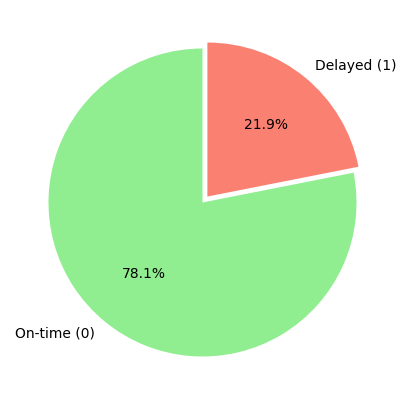
\includegraphics[width=0.4\textwidth]{Img/target_distribution.png}
    \caption{Flight Delay Distribution}
    \label{fig:line_sp}
\end{figure}
\subsection{Feature Distributions}
The numerical variables show a mix of skewed and balanced distributions.
\begin{itemize}
\item \textbf{Unbalanced features:}
\begin{itemize}
    \item \texttt{CRS\_DEP\_TIME} and \texttt{CRS\_ARR\_TIME} have visible peaks during morning and evening hours, reflecting flight scheduling patterns.
    \item \texttt{DISTANCE} is right-skewed, dominated by short- to mid-range routes but with a few long-haul flights.
\end{itemize}

\item \textbf{Balanced features:}
\begin{itemize}
    \item \texttt{MONTH}, \texttt{DAY\_OF\_MONTH}, and \texttt{DAY\_OF\_WEEK} are evenly distributed, showing consistent flight activity across time.
    \item Weather-related variables \texttt{HourlyDryBulbTemperature, HourlyDewPointTemperature, HourlyRelativeHumidity, HourlyWindSpeed} display near-normal patterns, indicating stable weather conditions.
\end{itemize}
\end{itemize}

The categorical features are highly imbalanced.
\begin{itemize}
\item The variable \texttt{OP\_UNIQUE\_CARRIER} shows that Alaska Airlines (AS) operates the majority of flights, followed by SkyWest (OO) and Delta (DL).

\begin{figure}[H]
    \centering
    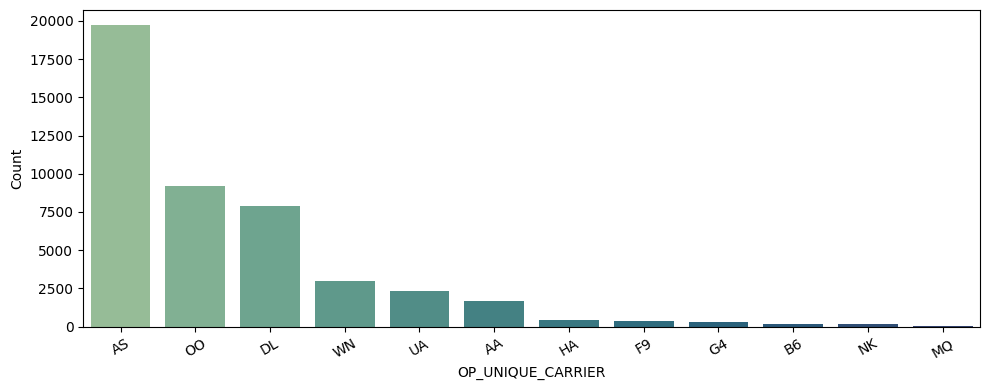
\includegraphics[width=0.7\textwidth]{Img/OP_UNIQUE_distribution.png}
    \caption{Airline Distribution}
    \label{fig:line_sp}
\end{figure}

\item From the \texttt{ORIGIN} variable, most flights in Washington depart from Seattle–Tacoma Airport (SEA), accounting for about 87.41\% of total flights.

\item The \texttt{DEST\_STATE\_ABR} distribution indicates that most destinations are in California (CA) (around 24.17\%), followed by Washington (WA) and Alaska (AK).
\end{itemize}
Overall, flight activity is mainly concentrated among a few major airlines, airports, and destination states.

\section{Bivariate Analysis}
Following the univariate exploration of both target and feature variables, this section extends the analysis to examine how these factors interact with flight delay outcomes. The bivariate investigation provides insights into how operational, temporal, and environmental conditions are associated with the likelihood of delays, offering a clearer picture of underlying patterns before model development.
\subsection{Operational Performance}

\begin{figure}[H]
    \centering
    % Ảnh bên trái
    \begin{subfigure}[b]{0.45\textwidth}
        \centering
        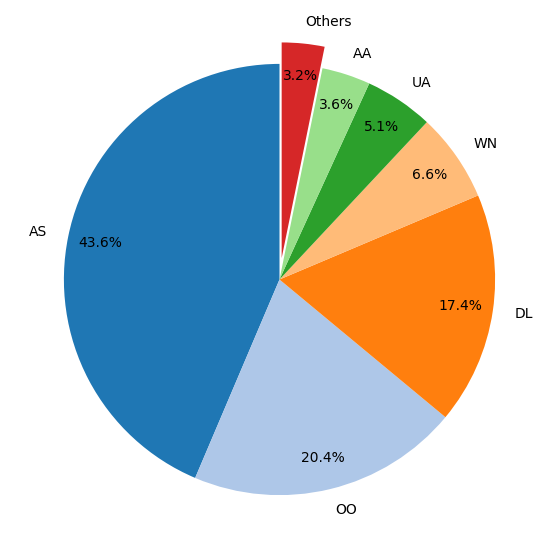
\includegraphics[width=0.6\textwidth]{Img/OPC_1.png}
        \caption{Airline distribution}
        \label{fig:Airline_distribution}
    \end{subfigure}
    \hfill
    % Ảnh bên phải
    \begin{subfigure}[b]{0.45\textwidth}
        \centering
        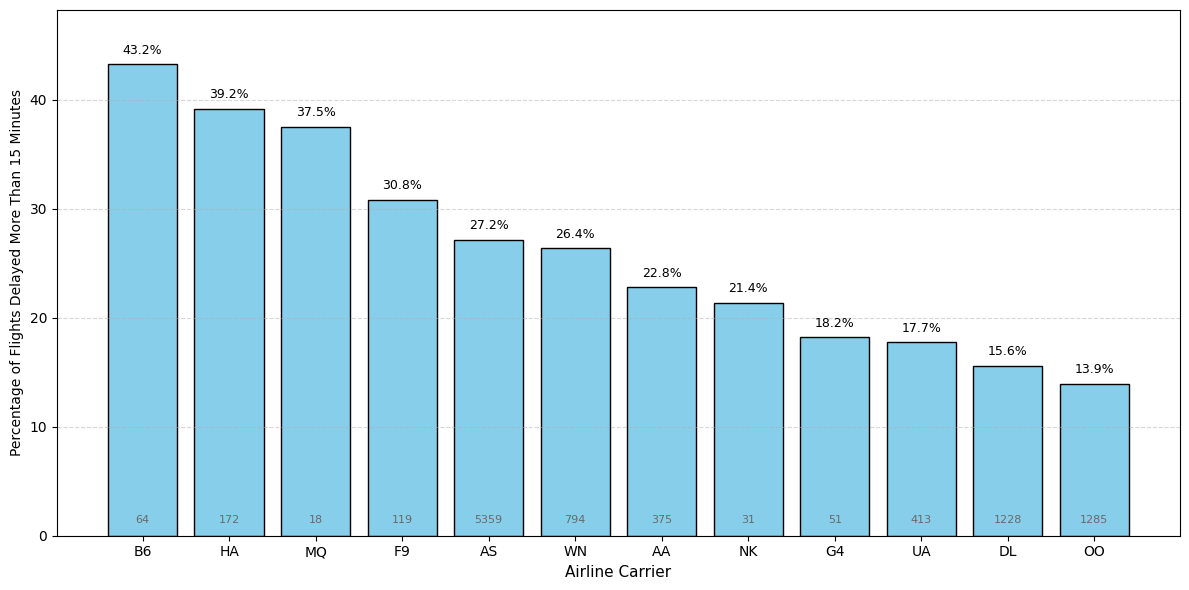
\includegraphics[width=\textwidth]{Img/OUC_2.png}
        \caption{Percentage of Flights Delayed More Than 15 Minutes by Airline}
        \label{fig:flights_Ariline}
    \end{subfigure}

    \caption{Airline operational overview showing flight distribution and delay rate performance}
    \label{fig:airline}
\end{figure}

As shown in Figure~\ref{fig:airline} provides an overview of airline operational performance, combining flight distribution and delay rate across carriers.
Alaska Airlines (AS) and SkyWest (OO) account for most flights in the dataset, reflecting their dominance in regional operations. However, delay rates differ notably among carriers. JetBlue (B6) and Hawaiian (HA) record the highest proportions of delayed flights, while SkyWest (OO) and Delta (DL) maintain better on-time performance.
These variations indicate differences in network efficiency and operational reliability. Large carriers with well-coordinated schedules experience fewer delays, whereas smaller or regional airlines are more affected by congestion, route length, and weather disruptions.


\begin{figure}[H]
    \centering
    % Ảnh bên trái
    \begin{subfigure}[b]{0.45\textwidth}
        \centering
        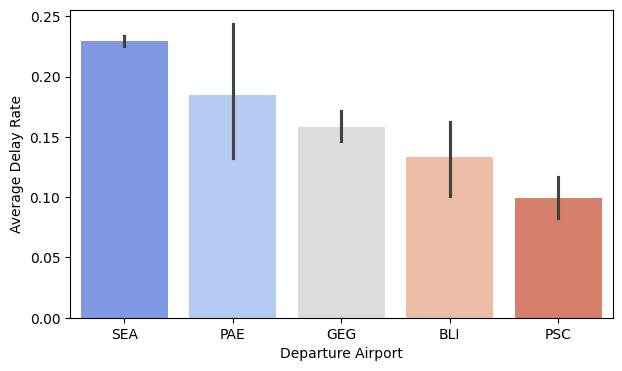
\includegraphics[width=0.85\textwidth]{Img/origin.png}
        \caption{Delay Rate by Departure Airport}
        \label{fig:origin}
    \end{subfigure}
    \hfill
    % Ảnh bên phải
    \begin{subfigure}[b]{0.45\textwidth}
        \centering
        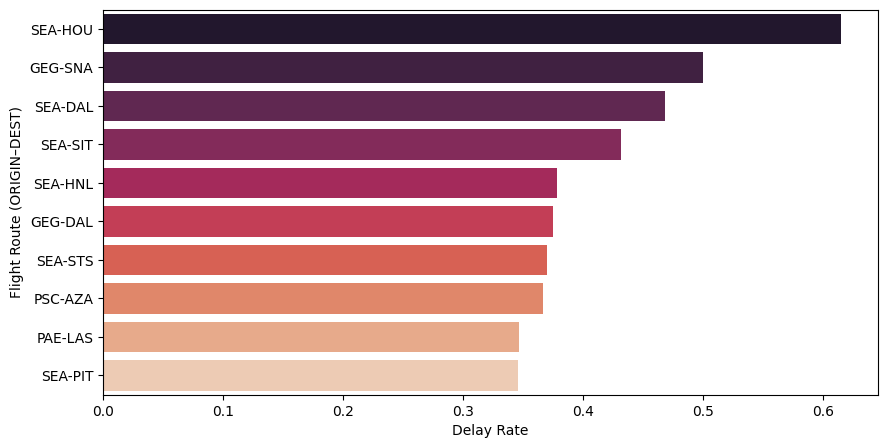
\includegraphics[width=\textwidth]{Img/origin_dest.png}
        \caption{Top 10 Routes with Highest Delay Rate}
        \label{fig:origin_dest}
    \end{subfigure}

    \caption{Flight delay patterns across airports and routes}
    \label{fig:ori}
\end{figure}

Figure~\ref{fig:ori} shows how flight delays vary across departure airports and routes.
Seattle (SEA) records the highest average delay rate, reflecting heavy traffic and hub congestion, while smaller airports like Pasco (PSC) and Bellingham (BLI) show better on-time performance.
Among flight routes, SEA–HOU and GEG–SNA exhibit the highest delay rates, exceeding 50\%, indicating that long-haul and hub-connected routes are more prone to disruptions.
Overall, the analysis suggests that airport size, route distance, and air traffic intensity play key roles in delay occurrence, with major hubs experiencing greater schedule pressure compared to smaller regional airports.

\begin{figure}[H]
    \centering
    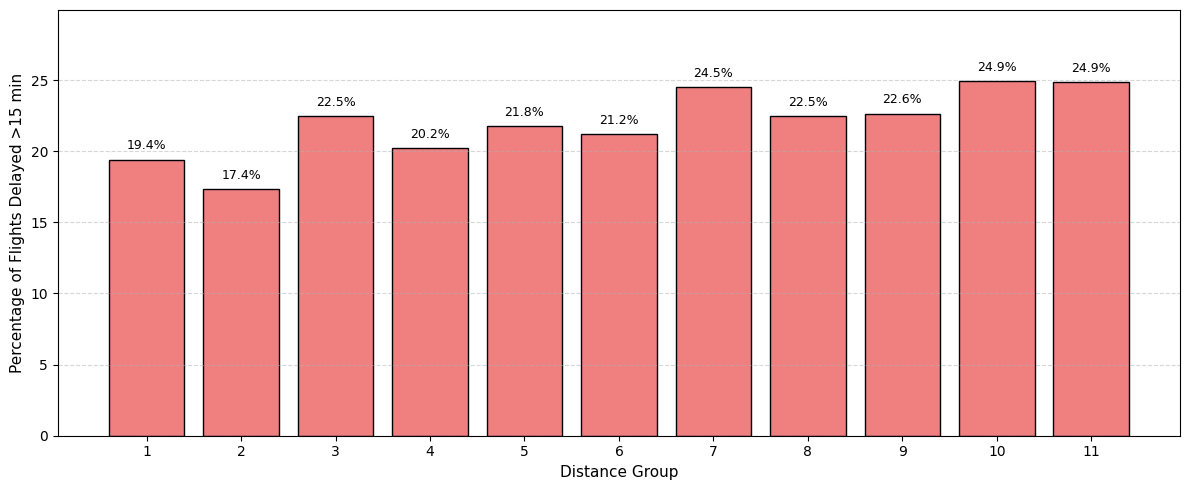
\includegraphics[width=0.8\textwidth]{Img/distance.png}
    \caption{Percentage of Flights Delayed more than 15 min by Distance Group}
    \label{fig:dis}
\end{figure}

According to Figure~\ref{fig:dis}, short-haul flights (Groups 1–3) show relatively low delay rates around 17–20\%, while medium- to long-haul flights (Groups 7–11) reach nearly 25\%.
This pattern suggests that longer routes are more exposed to operational disruptions such as air traffic control coordination, weather variations across regions, and limited flexibility in scheduling.
However, the difference is not extreme, implying that both short and long flights can experience delays depending on network congestion and turnaround efficiency.


Overall, the operational analysis shows that delay patterns are not evenly distributed across airlines, airports, or routes.
Major hubs and long-haul connections tend to experience higher delay rates, which may be caused by congestion, air traffic complexity, and tight scheduling.
Conversely, smaller carriers and regional airports maintain more stable on-time performance.
These findings suggest that operational capacity and traffic management could be key factors influencing flight punctuality.

\subsection{Temporal and Environmental Patterns}
Flight delays are often influenced not only by operational factors but also by when and under what conditions flights take place.
This part examines how delays vary throughout the day and week, and how weather elements such as wind speed or visibility contribute to schedule disruptions.
By combining temporal and environmental perspectives, the analysis helps identify periods and conditions where delays are more likely to occur.


\begin{figure}[H]
    \centering
    % Ảnh bên trái
    \begin{subfigure}[b]{0.45\textwidth}
        \centering
        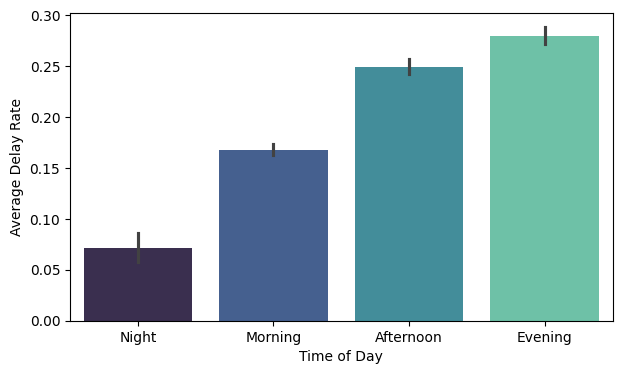
\includegraphics[width=\textwidth]{Img/time_of_day.png}
        \caption{Delay Rate by Time of Day}
        \label{fig:day}
    \end{subfigure}
    \hfill
    % Ảnh bên phải
    \begin{subfigure}[b]{0.45\textwidth}
        \centering
        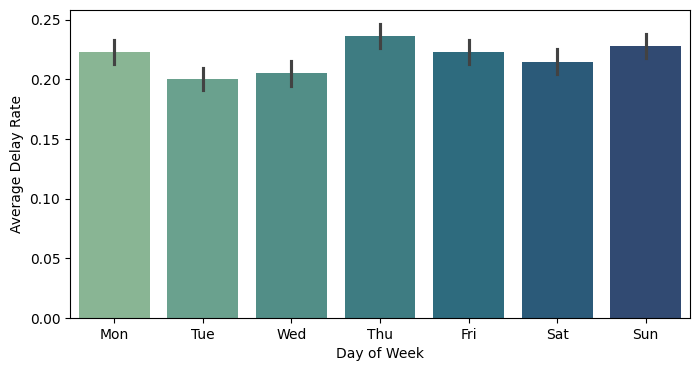
\includegraphics[width=\textwidth]{Img/day_of_week.png}
        \caption{Delay Rate by Day of Week}
        \label{fig:week}
    \end{subfigure}

    \caption{Temporal delay patterns by time of day and day of week}
    \label{fig:time}
\end{figure}

Figure~\ref{fig:time} presents temporal patterns of flight delays across different times of day and days of the week.
Delays increase steadily from morning to evening, with the highest average delay rate during evening flights, likely due to accumulated schedule disruptions and air traffic congestion throughout the day.
By contrast, night and early-morning flights show fewer delays, benefiting from lower traffic volumes and more stable operations.
Across the week, Thursdays and Sundays display slightly higher delay rates, possibly reflecting increased travel demand before weekends and at the end of the week.

\begin{figure}[H]
    \centering
    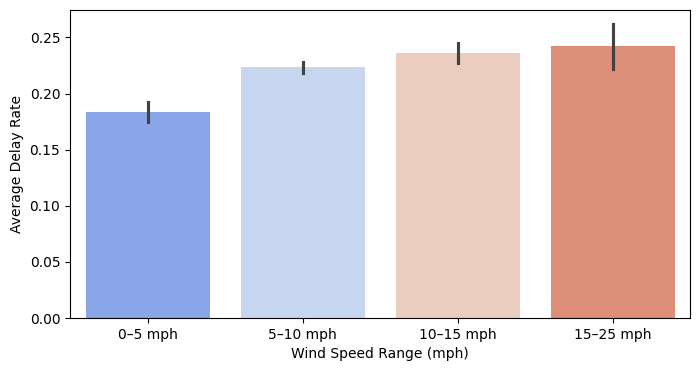
\includegraphics[width=0.8\textwidth]{Img/wind_group.png}
    \caption{Delay Rate by Wind Speed Group}
    \label{fig:wind}
\end{figure}


In Figure~\ref{fig:wind}, the delay rate gradually increases with wind speed, reaching its peak at 15–25 mph, when stronger crosswinds tend to slow down takeoff and landing operations.
These results indicate that both wind and visibility significantly affect operational efficiency.
Although modern navigation systems help mitigate such disruptions, adverse weather remains a major external factor that airlines must manage to maintain schedule reliability.

Overall, the temporal and weather analyses show that delays are more common during evening and late-week flights, reflecting higher traffic and schedule congestion.
Adverse weather, especially strong winds, further worsens punctuality.
These combined effects highlight that both timing and environmental conditions play key roles in shaping flight delay patterns.
\section{Correlation and Statistical Tests}
This section examines how flight operation and weather variables correlate with departure delay (\texttt{DEP\_DEL15}) and evaluates their statistical significance.

\begin{itemize}
\item \textbf{Correlation among Numerical Features}

The Pearson correlation results show that:
\begin{itemize}
    \item \texttt{CRS\_DEP\_TIME} has the highest positive correlation with delay ($r = 0.15, p < 0.001$), suggesting that later flights tend to be more delayed.
    \item Weather variables such as \texttt{HourlyDryBulbTemperature} and \texttt{HourlyWindSpeed} have very weak correlations ($r < 0.1$).
    \item \texttt{DISTANCE} and \texttt{CRS\_ELAPSED\_TIME} are highly correlated with each other but not with delay.
\end{itemize}

\begin{figure}[H]
    \centering
    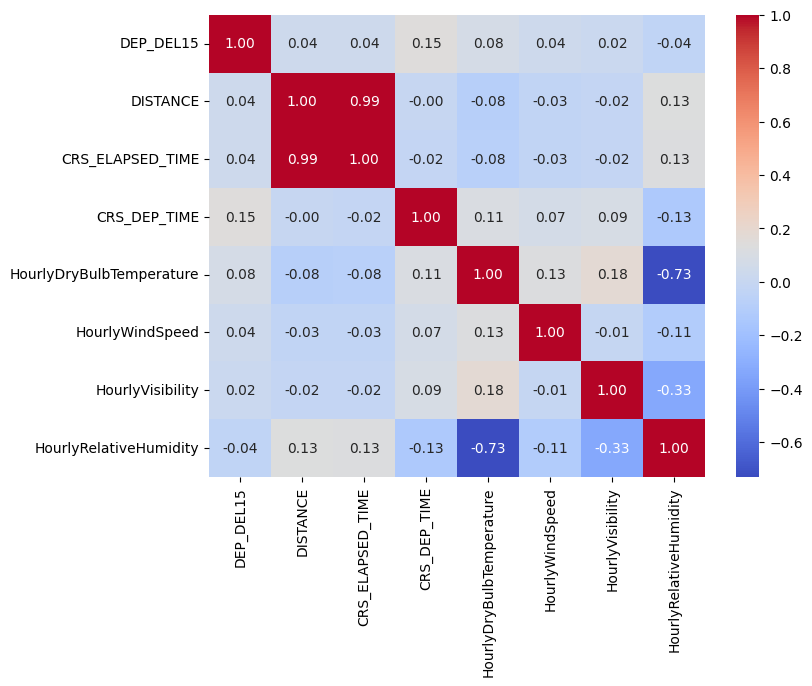
\includegraphics[width=0.7\textwidth]{Img/Correlation_Heatmap.png}
    \caption{Correlation Heatmap}
    \label{fig:line_sp}
\end{figure}

These results imply that \textbf{operational factors} (especially departure time) have a stronger linear effect on delay than \textbf{weather conditions}.

\item \textbf{Association between Categorical Features and Delay}

Chi-square tests confirm statistically significant relationships ($p < 0.001$) between delay occurrence and variables such as:
\begin{itemize}
    \item \texttt{OP\_UNIQUE\_CARRIER} -- delay rates vary across airlines.
    \item \texttt{ORIGIN} -- airports differ in on-time performance.
    \item \texttt{TIME\_OF\_DAY} and \texttt{MONTH} -- delays are more likely during specific hours or months.
\end{itemize}

This indicates that \textbf{delay frequency depends on both airline and scheduling factors}, not randomly distributed.

\vspace{1em}

\end{itemize}
In summary, correlation and hypothesis tests consistently highlight that \textbf{flight operation factors} (airline, airport, time of departure) significantly influence delay probability, while \textbf{weather features} show weak but statistically significant correlations.

\chapter{Modeling}
\section{Model Overview}
This study addresses flight delay prediction as a binary classification problem, aiming to determine whether a flight will be delayed by 15 minutes or more (DEP\_DEL15 = 1). The dataset integrates both operational and meteorological features, allowing the model to capture scheduling and weather effects simultaneously.

The modeling pipeline includes data splitting, feature scaling, imbalance handling, model training, and evaluation. Five machine learning models were implemented: Logistic Regression, KNN, Random Forest, XGBoost, and LightGBM. The F1-score was chosen as the primary evaluation metric to balance precision and recall in this imbalanced classification task.

\section{Data Preparation for Modeling}
Before model training, several preprocessing steps were applied to ensure data quality and compatibility with different algorithms. We use 80\% of our data for training and use the remaining 20\% for testing to evaluate the performance of our model.

Categorical variables such as airline, origin, and destination were encoded using Label Encoding. Numerical features were scaled depending on the model type: StandardScaler for Logistic Regression to to normalize feature magnitudes, and MinMaxScaler for K-Nearest Neighbors due to its distance sensitivity. Tree-based models (Random Forest, XGBoost, and LightGBM) were trained directly on unscaled feature.

To address the strong class imbalance between delayed and on-time flights, two strategies were employed: SMOTE oversampling to synthetically increase minority class, and model-based balancing. These steps ensured that each model could learn representative patterns and reduced bias toward the majority (non-delayed) class.

\section{Model Selection}
To identify the most suitable model for flight delay prediction, five supervised learning algorithms were evaluated: Logistic Regression, K-Nearest Neighbors (K = 3), Random Forest, XGBoost, and LightGBM.
These models represented different learning strategies—linear, distance-based, and ensemble methods—allowing for a comprehensive performance comparison.
\begin{itemize}

\item Logistic Regression served as a simple linear baseline model that estimates the probability of delay based on a weighted combination of input features.
\item K-Nearest Neighbors (K = 3) is a distance-based algorithm that classifies a flight by identifying the majority class among its nearest neighbors. It is effective for capturing local patterns but can be sensitive to feature scaling.
\item Random Forest is an ensemble method that combines multiple decision trees trained on random subsets of data and features. It helps reduce overfitting and improves prediction stability.
\item XGBoost and LightGBM are gradient boosting algorithms that build decision trees sequentially to correct previous errors. They are highly efficient, capable of modeling nonlinear relationships, and perform robustly on tabular data. LightGBM also includes built-in mechanisms to handle class imbalance effectively.
\end{itemize}

Each model was trained using the preprocessed dataset, with the appropriate scaling and imbalance-handling techniques applied. Hyperparameter tuning was performed using GridSearchCV with three-fold cross-validation, and the F1-score was chosen as the main evaluation metric because it balances precision and recall in imbalanced classification tasks.

After model training, an optimal decision threshold was determined for each model by maximizing the F1-score obtained from the precision–recall curve, instead of using the default probability cutoff of 0.5.

\chapter{Results and Discussion}

\section{Model Performance}

The performance of all models was evaluated using four main metrics: Precision, Recall, F1-score, and ROC-AUC. Since the dataset was highly imbalanced, with many more on-time flights than delayed ones, the F1-score was chosen as the main evaluation criterion. This score provides a balanced view of model performance by combining both precision and recall.
\begin{itemize}
    \item The F1-score is useful for imbalanced data because it does not depend only on accuracy, which can be misleading when one class dominates.
    \item In this study, recall was especially important. Detecting most delayed flights (high recall) is more valuable for airlines than avoiding false alarms (high precision), since early detection allows for better scheduling and passenger management.
\end{itemize}

\begin{table}[H]
\centering
\begin{adjustbox}{width=\textwidth}
\begin{tabular}{|c|c|c|c|c|c|}
\hline
\textbf{Model}  & \textbf{Precision} & \textbf{Recall} & \textbf{F1-score} & \textbf{ROC-AUC} \\
\hline
Logistic Regression & 0.29 & 0.65 & 0.40 & 0.64 \\
KNN (k=3) & 0.29 & 0.47 & 0.36 & 0.60 \\
Random Forest (default) & 0.38 & 0.24 & 0.30 & 0.66 \\
Random Forest (optimize) & 0.30 & 0.67 & 0.42 & 0.66 \\
XGBoost (default) & 0.45 & 0.20 & 0.28 & 0.68 \\
XGBoost (optimize )& 0.29 & 0.48 & 0.43 & 0.68 \\
LightGBM (default) & 0.34 & 0.66 & 0.45 & 0.71 \\
LightGBM (optimize) & \textbf{0.34} & \textbf{0.69} & \textbf{0.46} & \textbf{0.71} \\
\hline
\end{tabular}
\end{adjustbox}
\caption{Summary of model performance metrics}
\label{tab:model_performance}
\end{table}

Among all tested models, LightGBM achieved the highest recall and the best overall F1-score, making it the most effective model for practical flight delay prediction.
\begin{itemize}
    \item Its ability to detect a large number of delayed flights is valuable for real-world applications, even if precision remains moderate.
    \item This means the model is better at identifying potential delays, which is more useful for airlines that need early warnings rather than perfect accuracy.
\end{itemize}

\begin{figure}[H]
    \centering
    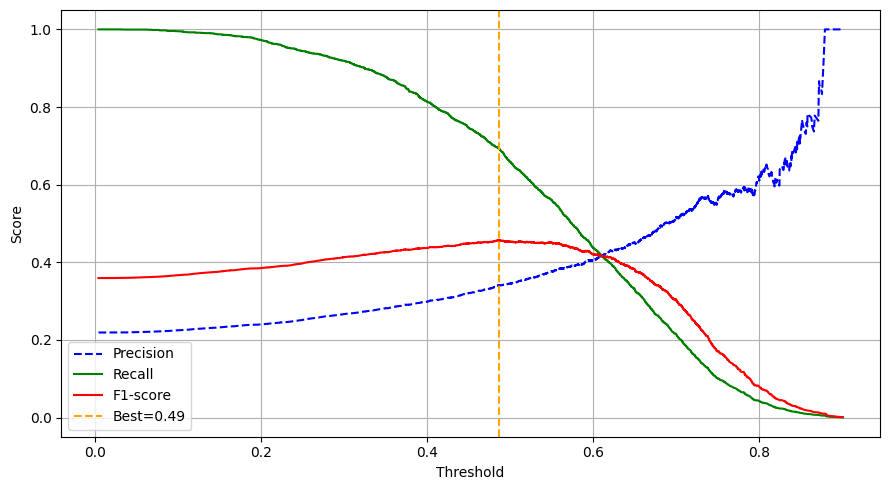
\includegraphics[width=0.8\textwidth]{Img/threshold_score.png}
    \caption{Precision–Recall–F1 curve for threshold optimization of the LightGBM model}
    \label{fig:optimized_threshold}
\end{figure}

After applying threshold optimization, the balance between precision and recall improved slightly. This adjustment allowed the model to maintain strong recall while increasing precision, leading to a more stable and reliable performance.

Overall, the optimized LightGBM model provided the best trade-off between sensitivity and prediction accuracy among all classifiers tested.

\section{Visualization and Discussion}

This section visualizes the performance of the LightGBM model using three plots: confusion matrix, ROC curve and feature importance. These figures help interpret how well the model distinguishes delayed flights and which features contribute most to its predictions.
    
\begin{figure}[H]
    \centering
    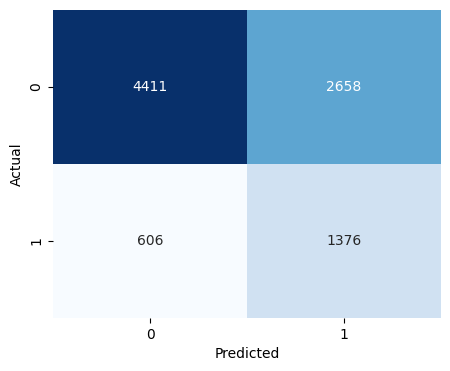
\includegraphics[width=0.8\textwidth]{Img/Confusion_matrix_L.png}
    \caption{Confusion Matrix of the LightGBM Model}
    \label{fig:confusion_matrix}
\end{figure}

The confusion matrix in  Figure~\ref{fig:confusion_matrix} shows the LightGBM model’s classification results after threshold optimization.
\begin{itemize}
    \item The model correctly predicted most on-time flights (4,411 true negatives) and successfully identified 1,376 delayed flights (true positives).
    \item However, 606 delayed flights were missed (false negatives), and 2,658 on-time flights were incorrectly classified as delayed (false positives).
\end{itemize}

This result explains the model’s high recall but relatively low precision, meaning it effectively detects delays but still raises some false alarms. This pattern can be explained by the imbalanced nature of the dataset, the influence of several operational factors such as aircraft inspections, boarding procedures, and airport congestion, and the fact that the LightGBM model was optimized to maximize recall, which naturally reduces precision.

\begin{figure}[H]
    \centering
    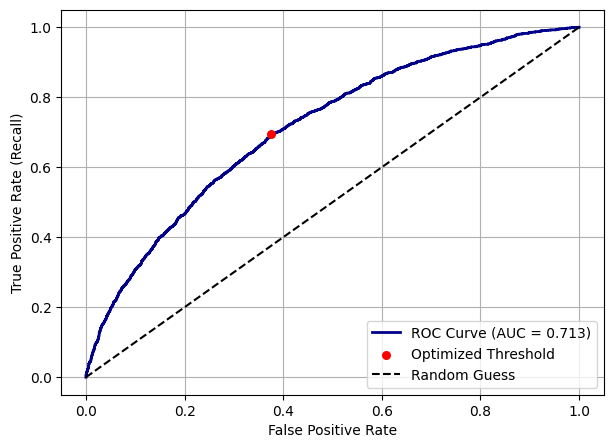
\includegraphics[width=0.8\textwidth]{Img/ROC.png}
    \caption{ROC curve of the LightGBM model}
    \label{fig:Roc}
\end{figure}

The ROC curve in Figure~\ref{fig:Roc} illustrates the trade-off between the True Positive Rate (Recall) and False Positive Rate across different thresholds.
\begin{itemize}
    \item The LightGBM model achieved an AUC of 0.713, indicating a fair ability to distinguish between delayed and on-time flights.
    \item The red point represents the optimized threshold ($\approx 0.49$) that maximizes the F1-score.
\end{itemize}

Although the curve does not reach very high sensitivity, it shows consistent predictive capability, suggesting that the model generalizes reasonably well despite data imbalance and operational variability.

\begin{figure}[H]
    \centering
    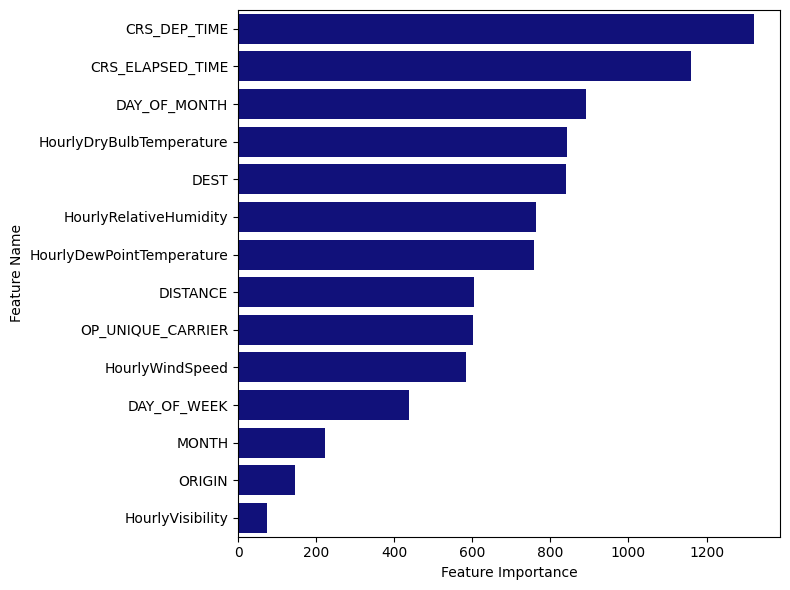
\includegraphics[width=0.8\textwidth]{Img/feature_im.png}
    \caption{ROC curve of the LightGBM model}
    \label{fig:features}
\end{figure}

    As shown in Figure~\ref{fig:features} presents the feature importance values from the LightGBM model.
\begin{itemize}
    \item The most influential variables are \texttt{CRS\_DEP\_TIME}, \texttt{CRS\_ELAPSED\_TIME}, and \texttt{DAY\_OF\_MONTH}.
    \item These scheduling features are followed by meteorological indicators such as \texttt{Humidity}, \texttt{DewPointTemperature} and \texttt{HourlyDryBulbTemperature}, which also play a significant role.
\end{itemize}

This suggests that both flight timing and environmental conditions are key determinants of delay occurrence, aligning with practical expectations in airline operations.

\section{Limitations and Future Work}
While the LightGBM model achieved the best overall performance with an F1-score of 0.46 and an AUC of 0.71, its precision remained relatively low. This reflects the challenge of predicting rare delay events and the trade-off between recall and precision in imbalanced datasets. Some influencing factors, such as real-time maintenance, crew scheduling, or air traffic control delays, were not included in the dataset, which limits the model’s ability to fully capture operational complexity. In addition, weather data were aggregated on an hourly basis, which may overlook short-term variations affecting flight punctuality. Despite these limitations, the model provides meaningful insights and a strong foundation for further improvement in airline delay prediction systems.


Although this project has successfully developed a predictive model and provided valuable analytical insights into flight delays, several directions can still be explored to further enhance and extend its scope in future research and development:

\begin{itemize}
    \item \textbf{Develop a real-time data pipeline} to automatically extract and process flight and weather information from public APIs, enabling continuous updates and near real-time predictions.
    \item \textbf{Enrich the dataset} with additional contextual features such as aircraft type, air traffic density, holiday indicators, or seasonal patterns to improve model performance.
    \item \textbf{Explore advanced and hybrid models} (e.g., ensemble or deep learning approaches) to enhance prediction accuracy and interpretability.
    \item \textbf{Deploy an interactive dashboard or API} to make the system accessible for end-users and support data-driven decision-making.
    \item \textbf{Automate retraining and monitoring} to ensure long-term adaptability of the model under changing flight and weather conditions.
\end{itemize}

\chapter*{Conclusion}

This study analyzed flight and weather data in Washington State to explore factors influencing departure delays. The results show that delays are not random but strongly linked to departure time and weather conditions such as visibility, humidity, and wind speed. These insights highlight how both operational and environmental factors shape flight punctuality.

By combining flight and weather datasets, the project built machine-learning models that can predict delays with good accuracy, with LightGBM performing best overall. The analysis provides useful information for improving flight scheduling and managing disruptions more proactively.

Finally, the work demonstrates how data engineering and machine learning can turn raw operational data into actionable insights. Future improvements may include extending the dataset and developing a real-time prediction pipeline for live delay monitoring.

\begin{thebibliography}{99}

\bibitem{btsdata}
Bureau of Transportation Statistics (BTS). \textit{Airline On-Time Performance Data}. U.S. Department of Transportation. Available at: \url{https://www.transtats.bts.gov/OT_Delay/OT_DelayCause1.asp}

\bibitem{noaa}
National Oceanic and Atmospheric Administration (NOAA). \textit{Integrated Surface Database (ISD): Hourly Weather Observations}. Available at: \url{https://www.ncei.noaa.gov/products/land-based-station/integrated-surface-database}

\bibitem{btsreport}
Bureau of Transportation Statistics. \textit{Understanding Airline Delays and Cancellations}. Washington, DC: U.S. Department of Transportation, 2023. Available at: \url{https://www.bts.gov/}

\bibitem{bregman2021}
Bregman, J., \& Hayashi, M. (2021). \textit{Flight Delay Prediction Using Machine Learning: A Data-Driven Approach}. \textit{Transportation Research Procedia}, 59, 383–392. \url{https://doi.org/10.1016/j.trpro.2021.06.044}

\bibitem{faa2010}
Ball, M., Barnhart, C., Dresner, M., Hansen, M., Odoni, A., \& Zou, B. (2010). \textit{Total Delay Impact Study: A Comprehensive Assessment of the Costs and Impacts of Flight Delay in the United States}. NEXTOR II Report, Federal Aviation Administration (FAA).

\bibitem{chandran2018}
Chandran, S., \& Sitaraman, R. (2018). \textit{Predicting Flight Delays Using Weather Data and Machine Learning Techniques}. In \textit{IEEE International Conference on Data Science and Advanced Analytics (DSAA)}.

\bibitem{nguyen2023}
Nguyen, P. T., \& Tran, D. H. (2023). \textit{Integrating Weather and Flight Operation Data for Delay Prediction Using Gradient Boosting Models}. \textit{Journal of Transportation and Logistics}, 10(2), 45–53.


\bibitem{lightgbm}
Ke, G., Meng, Q., Finley, T., et al. (2017). \textit{LightGBM: A Highly Efficient Gradient Boosting Decision Tree}. In \textit{Advances in Neural Information Processing Systems (NeurIPS)}.

\bibitem{nws}
National Weather Service (NWS). \textit{Aviation Weather Center: Understanding METAR and TAF Data}. Available at: \url{https://aviationweather.gov/}

\end{thebibliography}

\end{document}
